\begin{activity} \label{A:11.4.1} Suppose we want to find the area of the bounded region $D$ between the curves
\[y = 1-x^2 \ \ \ \ \ \text{ and } \ \ \ \ \ y=x-1.\]
A picture of this region is shown in Figure \ref{F:11.4.Area_ex_1}. 

\ba
	\item We know that the volume of a solid with constant height is given by the area of the base times the height.  Hence, we may interpret the area of the region $D$ as the volume of a solid with base $D$ and of uniform height 1.  Determine a double integral whose value is the area of $D$. 
\begin{figure}[ht]
\begin{center}
%\resizebox{!}{2.4in}{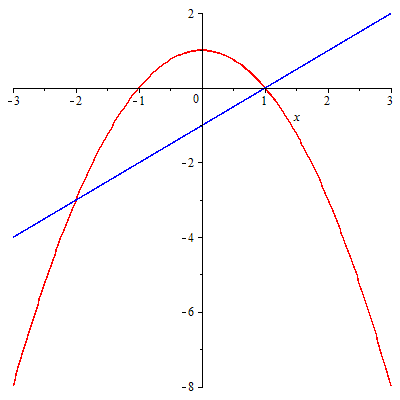
\includegraphics{11_4_Area_ex_1}}
  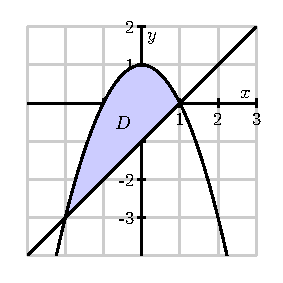
\includegraphics{figures/fig_11_4_area.eps}
\end{center}
\caption{The graphs of $y = 1-x^2$ and $y=x-1$.}
\label{F:11.4.Area_ex_1}
\end{figure}

	\item Write an iterated integral whose value equals the double integral you found in (a).
	\item Use the Fundamental Theorem of Calculus to evaluate \emph{only} the inner integral in the iterated integral in (b).  
	\item After completing part (c), you should see a standard single area integral from calc II. Evaluate this remaining integral to find the exact area of $D$.
\ea

\end{activity}
\begin{smallhint}

\end{smallhint}
\begin{bighint}

\end{bighint}
\begin{activitySolution}
\ba
\item The double integral
\[\int \int_D 1 \, dA\]
gives the volume of the solid of uniform height 1 and base area equal to the area of $D$, so this integral also gives the area of $D$. To set up this integral, we need to describe the region $D$. If we integrate with respect to $y$, then the graph of $y=1-x^2$ forms the top of $D$ and the graph of $y=x-1$ forms the bottom. To find the limits on $x$, we need to determine the points of intersections of the two curves. Now $y=1-x^2$ and $y=x-1$ intersect when $x^2+x-2 = (x-1)(x+2) = 0$ or when $x=-2$ and $x=1$. Therefore, the area of $D$ is given by the iterated integral
\[\int \int_D 1 \, dA = \int_{-2}^1 \int_{x-1}^{1-x^2} 1 \, dy \, dx.\]

\item The inner integral in our iterated integral is evaluated as 
\[\int_{x-1}^{1-x^2} 1 \, dy = y\bigm|_{x-1}^{1-x^2} = (1-x^2) - (x-1) = 2-x-x^2.\]

\item Completing the integration gives us
\begin{align*}
\int \int_D 1 \, dA &= \int_{-2}^1 \int_{x-1}^{1-x^2} 1 \, dy \, dx \\
	&= \int_{-2}^1 2-x-x^2 \, dx \\
	&= \left[2x-\frac{x^2}{2}-\frac{x^3}{3}\right]\biggm|_{-2}^1 \\
	&= \frac{7}{6} - \left(-\frac{10}{3}\right) \\
	&= \frac{9}{2}.
\end{align*}

\ea

\end{activitySolution}
\aftera
